\chapter{线性代数 - 克拉默法则}

\begin{figure}[ht]
  \centering
  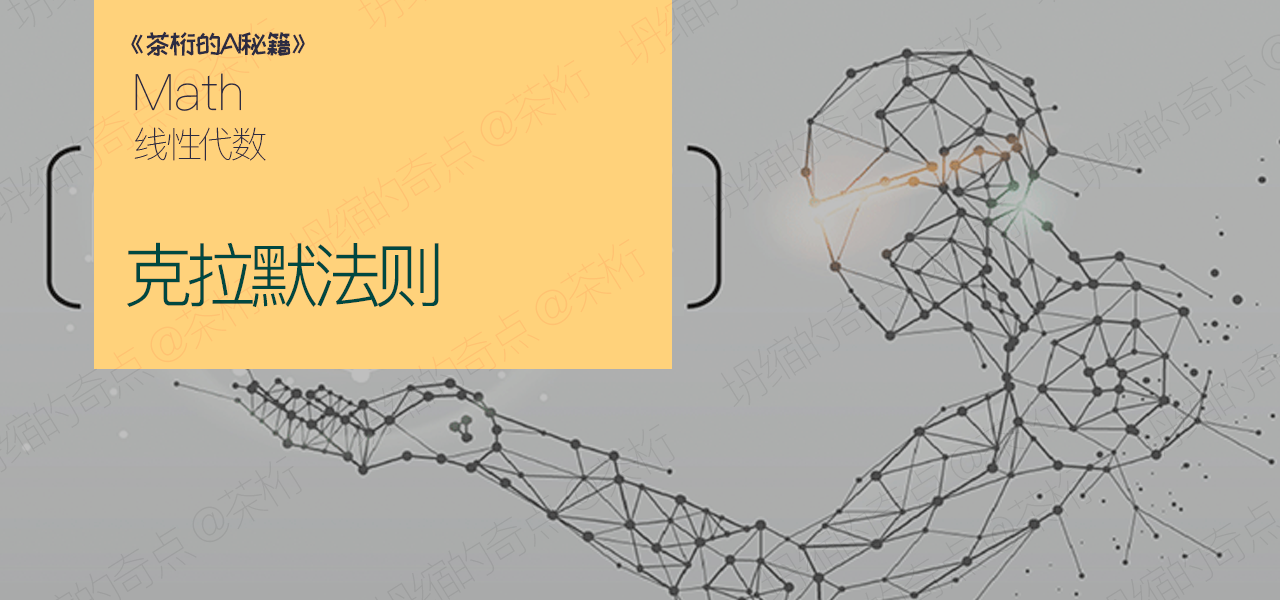
\includegraphics[width=1\linewidth]{asset/20230908142745.png}
\end{figure}

\newpage

上节课我们在最后提到了一个概念「\textit{克拉默法则}」, 本节课, 我们就来看看到底什么是克拉默法则. 

\hypertarget{15.线性代数}{}
\section{克拉默法则}

之前的课程我们一直在强调, 矩阵是线性方程组抽象的来的. 那么既然我们抽象出来了, 有没有一种比较好的办法高效的来求解这个线性方程组?不然抽象出来也没什么意义. 那么这个时候, 我们就引入了「克拉默法则」. 

克拉默法则是一种用于求解线性方程组的方法, 特别适用于方程组的系数矩阵是可逆的情况. 它允许我们通过计算矩阵的行列式和一系列辅助矩阵的行列式来找到方程组的解. 

我们前面的课程讲过, 一个线性方程组可以表示成这样: 

\[
  A_x = b
\]

其中, $A$是系数矩阵, $x$是未知量向量, $b$是常数向量: 

\[
  A = 
  \begin{bmatrix}
  a_1 \quad b_1 \quad c_1 \quad  d_1 \\
  a_2 \quad b_2 \quad c_2 \quad  d_2 \\ 
  a_3 \quad b_3 \quad c_3 \quad  d_3 \\
  a_4 \quad b_4 \quad c_4 \quad  d_4 \\
  \end{bmatrix}, \quad
  x = 
  \begin{bmatrix}
  x_1 \\
  x_2 \\
  x_3 \\
  x_4
  \end{bmatrix}, \quad
  b = 
  \begin{bmatrix}
  e_1 \\
  e_2 \\
  e_3 \\
  e_4
  \end{bmatrix}
\]

它计算时先用第一行的系数${a1, b1, c1, d1}$分别去乘以向量$x$里的列项, 就会是$a_1 \cdot x_1$, $b_1 \cdot x_2$, $c_1 \cdot x_3$, $d_1 \cdot x_4$ , 然后加在一起得到了$e_1$. 下面的行也依次这么计算, 得到$e_2 ,e_3 ,e_4 $. 

我们来考虑一个包含n个线性方程和n个未知数的线性方程组: 

\begin{align*}
  & a_{11}x_1 + a_{12}x_2 + ... + a_{1n}x_n = b_1 \\
  & a_{21}x_1 + a_{22}x_2 + ... + a_{2n}x_n = b_2 \\
  & \vdots \\
  & a_{n1}x_1 + a_{n2}x_2 + ... + a_{nn}x_n = b_n
\end{align*}

其中, $a_{ij}$是系数矩阵的元素, $x_i$是未知数, $b_i$是右侧的常数项. 

我们先要计算系数矩阵$A$的行列式$|A|$. 系数矩阵$A$是一个$n \times n$的矩阵, 其元素为$a_{ij}$, 行列式的计算可以使用一下公式:

\[
  |A| = \sum_{i=1}^n(-1)^{i+j}a_{ij}|M_{ij}|
\]

这个式子我们在之前讲N阶行列式的时候有讲过. 其中$M_{ij}$是剔除第$i$行和第$j$列后的子矩阵的行列式. 也就是说, $M_{ij}$是一个$(n-1) \times (n-1)$的矩阵. 

接着我们就需要创建辅助矩阵. 我们需要创建n个辅助矩阵$A_1,A_2,..., A_n$, 这些矩阵是将系数矩阵$A$列中的每一列替换成常数项矩阵$[b_1,b_2,..., b_n]$后得到的矩阵. 

\begin{align*}
  A_1 =
  & \begin{bmatrix}
  b_1 \quad a_{12} \quad \cdots \quad a_{1n} \\
  b_2 \quad a_{22} \quad \cdots \quad a_{2n} \\
  \vdots \quad \vdots \quad \ddots \quad \vdots \\
  b_n \quad a_{n2} \quad \cdots \quad a_{nn}
  \end{bmatrix} \\
  A_2 =
  & \begin{bmatrix}
  a_{11} \quad b_1 \quad \cdots \quad a_{1n} \\
  a_{21} \quad b_2 \quad \cdots \quad a_{2n} \\
  \vdots \quad \vdots \quad \ddots \quad \vdots \\
  a_{n1} \quad b_n \quad \cdots \quad a_{nn}
  \end{bmatrix} \\
  & \qquad \vdots\\
  A_n =
  & \begin{bmatrix}
  a_{11} \quad a_{12} \quad \cdots \quad b_1 \\
  a_{21} \quad a_{22} \quad \cdots \quad b_2 \\
  \vdots \quad \vdots \quad \ddots \quad \vdots \\
  a_{n1} \quad a_{n2} \quad \cdots \quad b_n
  \end{bmatrix} \\
\end{align*}

得到以上这个矩阵之后, 就需要来计算辅助矩阵的行列式$|A_1|, |A_2|,..., |A_n|$. 计算这些辅助矩阵的行列式. 你可以使用相同的方法, 即对每个辅助矩阵$A_i$, 使用与步骤1中相似的公式计算行列式. 

接下来我们就可以计算未知数的值, 通过以下公式计算: 

\begin{align*}
  x_1 = \frac{|A_1|}{|A|}, \quad x_2 = \frac{|A_2|}{|A|}, \quad ..., \quad x_n = \frac{|A_n|}{|A|}
\end{align*}

这些值就是线性方程组的解. 

需要注意的是, 克拉默法则要求系数矩阵$A$的行列式$|A|$不等于零, 否则无法使用克拉默法则来求解线性方程组. 如果$|A| = 0$, 则克拉默法则无法应用, 因为这意味着线性方程组可能没有唯一解或没有解. 此外, 克拉默法则在实际计算中可能不如其他方法高效, 因此对于大规模的方程组, 通常会使用其他数值方法来求解. 

我们变换上方的式子, 写成$x_i = \frac{|A_i|}{|A|}$, 在这个式子中, $|A_i|$就是把$|A|$中第$i$列元素换成常数向量, 而其余各列保持不变的到的. 

比如我们说$x_1$, 那我们就是将$|A|$的第一列, 也就是${a_1, a_2, a_3, a_4}$给它换成常数向量, 就变成${e_1, e_2, e_3, e_4}$, 其余的部分保持不变. 

那我们现在就需要计算新组合成的矩阵的值: 

\begin{align*}
  \begin{bmatrix}
  e_1 \quad b_1 \quad c_1 \quad  d_1\\
  e_2 \quad b_2 \quad c_2 \quad  d_2\\ 
  e_3 \quad b_3 \quad c_3 \quad  d_3\\
  e_4 \quad b_4 \quad c_4 \quad  d_4\\
  \end{bmatrix}
\end{align*}


同理$x_2,x_3,x_4$也是样子去得到的. 

克拉莫法则就是告诉我们$x_1,x_2,x_3$怎么求, 就是把系数矩阵的行列式值求出来然后再构造这么一个矩阵, 要求第几个未知量就把第几列系数矩阵里面第几列给它替换成$b$, 然后再算它行列式的值就可以了. 

克拉默法则有一些相关性质需要记住:

第一是我们之前提到的, 当系数行列式不等于$0$时, 方程组有唯一解, 当然这一条并不是绝对的. 当方程组是线性无关的, 即方程组中的方程不可以通过线性组合得到其他方程. 如果不满足这个条件, 即方程组中的方程之间存在线性相关性, 那么即使$|A| \ne 0$, 克拉默法则也无法确保方程组有唯一解. 

我们说回不等于0时方程组有唯一解, $a$的行列式的值出现在分母上的, 你不等于0的话分式的值是唯一的, 不会变的, 只有唯一的一个情况. 但是如果等于0的话那就说不清了, 有可能无解, 也有可能有很多个解. 

对于奇次线性方程组, 其有非零解的充要条件为其系数行列式为$0$, 其仅有零解的充要条件为其系数行列式不为$0$. 零解就是各个解$x_1,x_2, x_3, ...$, $x_i$全部为0叫做零解. 

还有一点就是, 当方程组中方程的个数与未知量的个数不同时, 抑或系数行列式为$0$时, 克拉默法则失效. 

我们来看一个实际的例子, 还是鸡兔同笼的问题, 我们就用克拉默法则求解及图同笼问题, 看一下克拉默法则如何解决实际问题. 

鸡和兔子同笼, 一共有35个头和94只脚, 问鸡和兔子各多少只. 

先把方程组列出来: 

\begin{align*}
& \begin{cases}
x + y = 35 \\
2x + 4y = 94
\end{cases}
\Rightarrow
A = 
\begin{bmatrix}
1 & 1 \\
2 & 4
\end{bmatrix},
X = \begin{bmatrix}x \\ y \end{bmatrix}, 
b = \begin{bmatrix} 35 \\ 94 \end{bmatrix}
\end{align*}

这样, 我们就将系数矩阵, 未知量以及常数量分别抽象出来. 接着我们来尝试进行计算: 

\begin{align*}
  & |A| = 1 \times 4 - 1 \times 2 = 2 \ne 0 \\
  x &  = \frac{|A_1|}{|A|} = \frac{\begin{vmatrix} 35 \quad 1 \\ 94 \quad 4 \end{vmatrix}}{2} = \frac{46}{2} = 23, \\
  y & = \frac{|A_2|}{|A|} = \frac{\begin{vmatrix} 1 \quad 35 \\ 2 \quad 94 \end{vmatrix}}{2} = \frac{24}{2} = 12
\end{align*}

那我们现在就得到了, 23只鸡, 12只兔子. 

现在我们得出的结果和消元法得到的结果是一样的, 所以克拉默法则给我们用行列式的方法求解线性方程组提供了一个新的思路. 

\section{矩阵运算}

在看完克拉默法则之后, 咱们再来看看关于矩阵运算的内容. 其实我们在导论课里面有提到, 因为它是非常基础的内容, 所以我们这里再给大家回顾一下, 矩阵的加减法非常简单. 

矩阵的加减法必须两个矩阵是同等大小的, 行数和列数都必须相同, 才能去做加减法运算. 其运算是在对应位置上的元素去做运算, 也就是左上角和左上角运算, 右下角和右下角运算. 那n行m列, 就必须和n行m列进行运算. 如下: 

\begin{align*}
\begin{bmatrix}
a_{11} \quad a_{12} \\
a_{21} \quad a_{22}
\end{bmatrix}
+
\begin{bmatrix}
b_{11} \quad b_{12} \\
b_{21} \quad b_{22}
\end{bmatrix}=
\begin{bmatrix}
a_{11} + b_{11} \quad a_{12} + b_{12} \\
a_{21} + b_{21} \quad a_{22} + b_{22}
\end{bmatrix} \\ \\
\begin{bmatrix}
a_{11} \quad a_{12} \\
a_{21} \quad a_{22}
\end{bmatrix}
-
\begin{bmatrix}
b_{11} \quad b_{12} \\
b_{21} \quad b_{22}
\end{bmatrix}=
\begin{bmatrix}
a_{11} - b_{11} \quad a_{12} - b_{12} \\
a_{21} - b_{21} \quad a_{22} - b_{22}
\end{bmatrix}
\end{align*}

这两个运算非常简单, 也非常容易理解, 我就不多说了, 大家看一下就行. 

然后就是矩阵的另外两种运算, 一个标量乘法, 一个向量乘法. 

矩阵的「标量」乘法就是拿一个常数和矩阵去乘: 

\begin{align*}
C \times
\begin{bmatrix}
b_{11} \quad b_{12} \\
b_{21} \quad b_{22}
\end{bmatrix}=
\begin{bmatrix}
Ca_{11} \quad Ca_{12} \\
Ca_{21} \quad Ca_{22}
\end{bmatrix}
\end{align*}

「\textbf{向量乘法}」, 是非常重要的一个乘法. 我们在神经网络里面无论是前向传播还是反向传播的时候, 向量乘法都是大量使用的. 不然上一层的值没办法传到下一层, 这些看似简单东西, 构起了整个知识体系的一个基石. 

向量乘法要求第一个矩阵的列数和第二个矩阵的行数必须相等. 如果第一个矩阵是两列, 这第二个矩阵必须是两行. 基于这样一个要求, 我相信小伙伴们也猜出来了, 它就是拿行去乘以列的一个运算. 第一个矩阵的元素一行一行的取出来, 第二个矩阵的元素以列一列的取出来, 然后进行乘积: 

\begin{align*}
\begin{bmatrix}
a_{11} \quad a_{12} \\
a_{21} \quad a_{22}
\end{bmatrix}
\times
\begin{bmatrix}
b_{11} \quad b_{12} \\
b_{21} \quad b_{22}
\end{bmatrix}=
\begin{bmatrix}
a_{11}b_{11} + a_{12}b_{21} \quad a_{11}b_{12} + a_{12}b_{22} \\
a_{21}b_{11} + a_{22}b_{21} \quad a_{21}b_{12} + a_{22}b_{22}
\end{bmatrix}
\end{align*}

那这个是一个$2 \times 2$的行列式进行乘积, 如果是一个$4 \times 3$的矩阵和一个$3 \times 5$的矩阵做一个向量乘法, 会得到几行几列呢?答案是$4 \times 5$. 

那以上就是我们本节课的内容, 相对来说, 这节课算是比较简单的. 大家要好好去巩固一下自己还不太熟悉的部分, 因为下一节课要进入神经网络了. 咱们一起来看看「神经网络中的矩阵/向量」. 并在此基础之上, 再好好讨论一下矩阵的性质. 
